\documentclass{standalone}
\usepackage{pgf}
\usepackage{amsmath}
\usepackage{tikz}
\usetikzlibrary{shapes,arrows}
\usetikzlibrary{positioning}
\begin{document}
   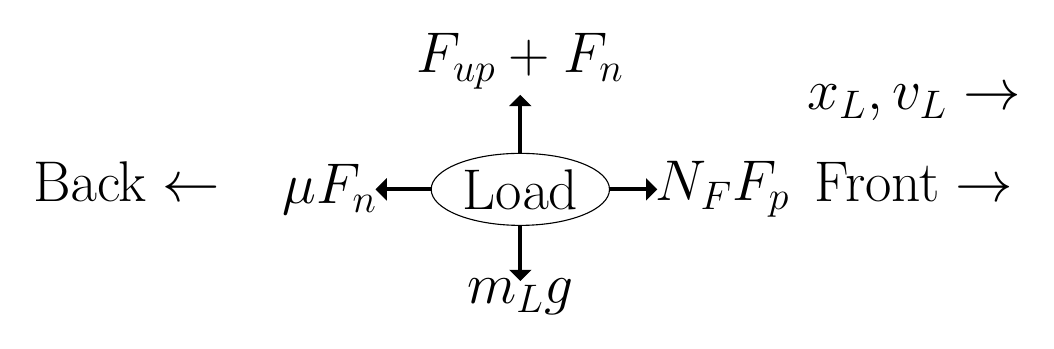
\begin{tikzpicture}[
    node distance = 0mm,
every node/.style = {inner sep=2pt}]
\coordinate                     (a)  at (0,0);
\coordinate[below=11mm of a]    (b);

\node[ellipse,draw,minimum size=3mm, 
      at=(b)]            (c)    {\huge Load};
  


\node[above=1mm of a]         {\huge $F_{up}+F_n$};
\path[draw=black,solid,line width=0.5mm,fill=black,
preaction={-triangle 90,thin,draw,shorten >=-1mm}
] (c) -- (a);


\node[right=5mm of c]  (d)       {\huge $N_F F_p$};
\path[draw=black,solid,line width=0.5mm,fill=black,
preaction={-triangle 90,thin,draw,shorten >=-1mm}
] (c) -- (d);

\node[left=6mm of c]  (e)       {\huge $\mu F_n$};
\path[draw=black,solid,line width=0.5mm,fill=black,
preaction={-triangle 90,thin,draw,shorten >=-1mm}
] (c) -- (e);


\node[below=6mm of c]  (f)       {\huge $m_L g$};
\path[draw=black,solid,line width=0.5mm,fill=black,
preaction={-triangle 90,thin,draw,shorten >=-1mm}
] (c) -- (f);


\node  (g) at (5,-1)       {\huge $ \text{Front} \rightarrow$};
\node  (x) at (5,0)       {\huge $ x_L,v_L \rightarrow$};
\node (h) at (-5,-1)       {\huge $ \text{Back} \leftarrow$};



%\node[above left =of a]  (d)    {$\downarrow W_m$};
%\node[above=of d.north west]    {$\uparrow^+$};
    \end{tikzpicture}
\end{document}
